\documentclass[conference]{IEEEtran}
\usepackage[utf8]{inputenc}
\usepackage{amsmath}
\usepackage{units}
\usepackage{graphicx}
\usepackage{multirow}
\usepackage{comment}
\usepackage{listings}
\usepackage{placeins}
\usepackage{float}
\usepackage{hyperref}\usepackage[utf8]{inputenc}

\begin{document}

\title{Exploring Feature Engineering and Various Machine
Learning Models for Human Action Recognition on the
UTD-MHAD}

\author{\IEEEauthorblockN{Alfred Tay
Wenjie\IEEEauthorrefmark{1},
Wang Zilong\IEEEauthorrefmark{2}, and Wong Yoke
Keong\IEEEauthorrefmark{3} } \\
\IEEEauthorblockA{Institute of Systems Science, National
University of Singapore \\
Email: e0402082@u.nus.edu\IEEEauthorrefmark{1},
e0402064@u.nus.edu\IEEEauthorrefmark{2},
e0384996@u.nus.edu\IEEEauthorrefmark{3},
}}
\maketitle

\date{September 2019}

\begin{abstract}
This paper sets out to explore sensor-based machine learning approaches to human activity recognition. Through studying the human anatomy and how the human body moves to perform various actions, feature engineering was carried out to extract distinctive information from the dataset and to remove variances that distracts the classification of human actions. The feature engineered dataset was fed into various machine learning and deep learning models and two of the models has outperformed the benchmark accuracy set by the collaborative representation classifier. A new graph machine learning model was conceptualised and implemented from scratch and has achieved high accuracy in classifying a subset of the 27 actions. Lastly, an image classification approach was explored by encoding the dataset into images and leveraging transferred learning model to perform the classification.  
\end{abstract}

\section{Introduction}
Human Activity Recognition has been one of the key research areas in recent history with the focus of observing and recognizing actions and goals of individuals or agents inside an environment. This task has wide-ranging applications in industries like Healthcare and Security. One application of the team's interest is the task of recognizing aggressive human behavior in in-door areas where security is highly valued. This allows building security teams to act quickly to contain the behaviors of miscreants, causing less damage and harm to people and properties.

In this assignment, the team sets out to explore sensor-based machine learning approaches to human activity recognition. An area of focus include engineering of features based on the team's understanding of the unique properties of sensors used and how they relate to the human anatomy and movements and the application of ensemble machine learning methods and LSTM models commonly used with time-series data.

In addition, the team also seeks to explore alternative representations and methods less commonly used for Human Activity Recognition including pattern recognition using graph-based machine learning models and the use of imaging methods to encode time series.

The team selected the Human Activity Recognition Dataset described in the 2015 paper 'UTD-MHAD: A Multimodal Dataset for Human Action Recognition Utilizing a Depth Camera and a Wearable Inertial Sensor' by Chen et al \cite{UTD-MHAD}. This dataset has been selected due to the multi-modal sensor data (e.g. Skeleton, Video, Inertial) available and the large variety of actions recorded (27-classes) available for exploration and training. Mentioned in the same paper, collaborative representation classifier was used to classify the 27 activities with an overall accuracy of 79.1 percent.


\section{Understanding the Dataset}

The 27 different actions were performed by 8 subjects (4 females and 4 males). Each subject repeated each action 4 times producing 32 samples per action. After removing three corrupted sequences, the dataset contains 861 data sequences. Four data modalities of RGB videos, depth videos, skeleton joint positions, and the inertial sensor signals were recorded in three channels or threads.

In this exploration, we would only be using the inertial
and skeleton dataset. We split the
train-validation data in the same fashion as the original
paper \cite{UTD-MHAD}, where subjects 1, 3, 5, 7 would be
used for training and subjects 2, 4, 6, 8 for validation,
so that we could perform a baseline comparison.

Splitting the dataset in this manner makes training a machine learning model very challenging as there is only 16 samples per action for the model to learn from and the validation is done against actions performed by subjects unseen by the model. Intuitively, different subjects will carry out the same action in a slightly different manner and the model had to be able to generalise based on just learning from 16 sample data on 27 actions with varying degrees of similarity.  

It was also noted that the 861 data sequences has different frame size due to the difference in duration of the subjects carrying out the various actions. 

\section{Feature Engineering}

Feature engineering was carried out with the main aim to
extract distinctive information from the data and to
remove variance that distracts the classification task.
Specifically, for the skeleton dataset, the unwanted
variance is the limbs and body length and the speed of
movement in executing the various actions. 

\subsection{Joint Angles}
The skeleton data contains joint position data in 3D
Cartesian Coordinate System. For different people, the
data points for the same action will be very different due
to differences in limbs and body length. Skeleton Joint Angles on the other hand offers more consistent data points for
different people executing the same action. The joint
angle is computed by finding the angle between 2 lines using the formula below.

\begin{equation}
Angle = \arccos{\frac{a\cdot b}{||a|| \cdot ||b||}}
\end{equation}


A total of 16 joint angles as depicted in fig \ref{fig:SkeletonJoints} has been defined and computed.

\begin{figure}[H]
\begin{center}
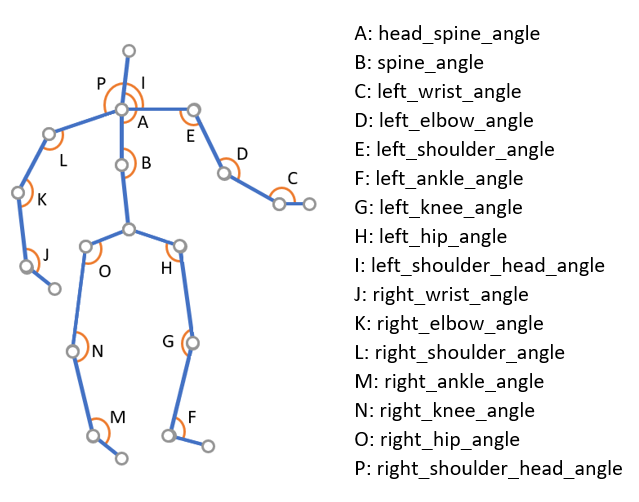
\includegraphics[scale=0.6]{Image/Skeleton_Joints.png}
\caption{\label{fig:SkeletonJoints} Skeleton Joints}
\end{center}
\end{figure}

\subsection{Variance in Joint Angles}

The variance within each of the joint angle value over the
entire sampling period was computed. 

\subsection{Variance in Inertial Sensor}

The variance for each inertial sensor data point over the entire
sampling period was computed. 

\subsection{Joint Angle Displacement}

The total joint angle displacement for each joint angle
over the entire sampling period was computed using the
formula below.

\begin{equation}
Total Joint Angle Displace = \sum |a_t - a_{t-1}|
\end{equation}


\subsection{Peak Count}

The total number of peak amplitudes are calculated for
joint angles and inertial sensor data. Peak detection
technique was used to identify the peaks in the signal. 

\begin{figure}[H]
\begin{center}
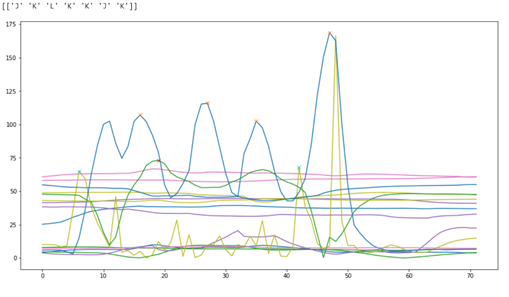
\includegraphics[scale=1]{Image/Peak_Detection.png}
\caption{\label{fig:Peak_Detection} Peak Detection for
Joint Angle Signal}
\end{center}
\end{figure}

\subsection{Joint Sequence}

Given that all movement is controlled by the joints, it
was hypothesized that the sequence of joint activation
will provide distinctive patterns for different actions.
The joint sequence for each sample is compiled by
identifying the sequence of peaks detected in each of the
16 joint angle signals. The joint sequence data removes the
unwanted variance in the speed of movement in the original
data.

Fig \ref{fig:Peak_Detection} shows the 16 joint angular changes for the right-hand wave action. The joint activation sequence complied is: right wrist angle, right elbow angle, right shoulder angle, right elbow angle, right elbow angle, right wrist angle, right elbow angle.

\section{Training Machine Learning Models}

After performing feature engineering, the team proceeded to apply several machine learning methods for comparison in search of good model performance. These machine learning models range from ensembles to neural networks and heterogeneous multi-classifiers.

For all the models in this section, the engineered features listed in table \ref{tbl:input_features} was used as the input dataset. Four of the skeleton joint angle signals, namely: left and right ankle angle and left and right head to shoulder angle, were not used as these joints tends to be activated sporadically across all the actions.    

\begin{table}[H] 
\begin{center}
\caption{Input Features} \label{tbl:input_features}
\begin{tabular}{|c|c|}
\hline
Feature Description & No. of Features \\
\hline
Variance within each of the joint angle signals  & 12  \\
\hline
Peak count for each of the  joint angle signals & 12  \\
\hline
Variance within each of the inertial sensor signals & 6  \\
\hline
Peak count for each of the inertial sensor signals & 6  \\
\hline
Total & 36  \\
\hline
\end{tabular}
\end{center}
\end{table}

\subsection{Random Forest}

When Random Forest was applied to the above dataset, an accuracy of 79.77 percent was achieved. It was observed that class 1 has the lowest f1-score of 0.24 and the confusion matrix showed that class 1 is most confused with class 0 (0.56 vs 0.44)

\begin{figure}[H]
\begin{center}
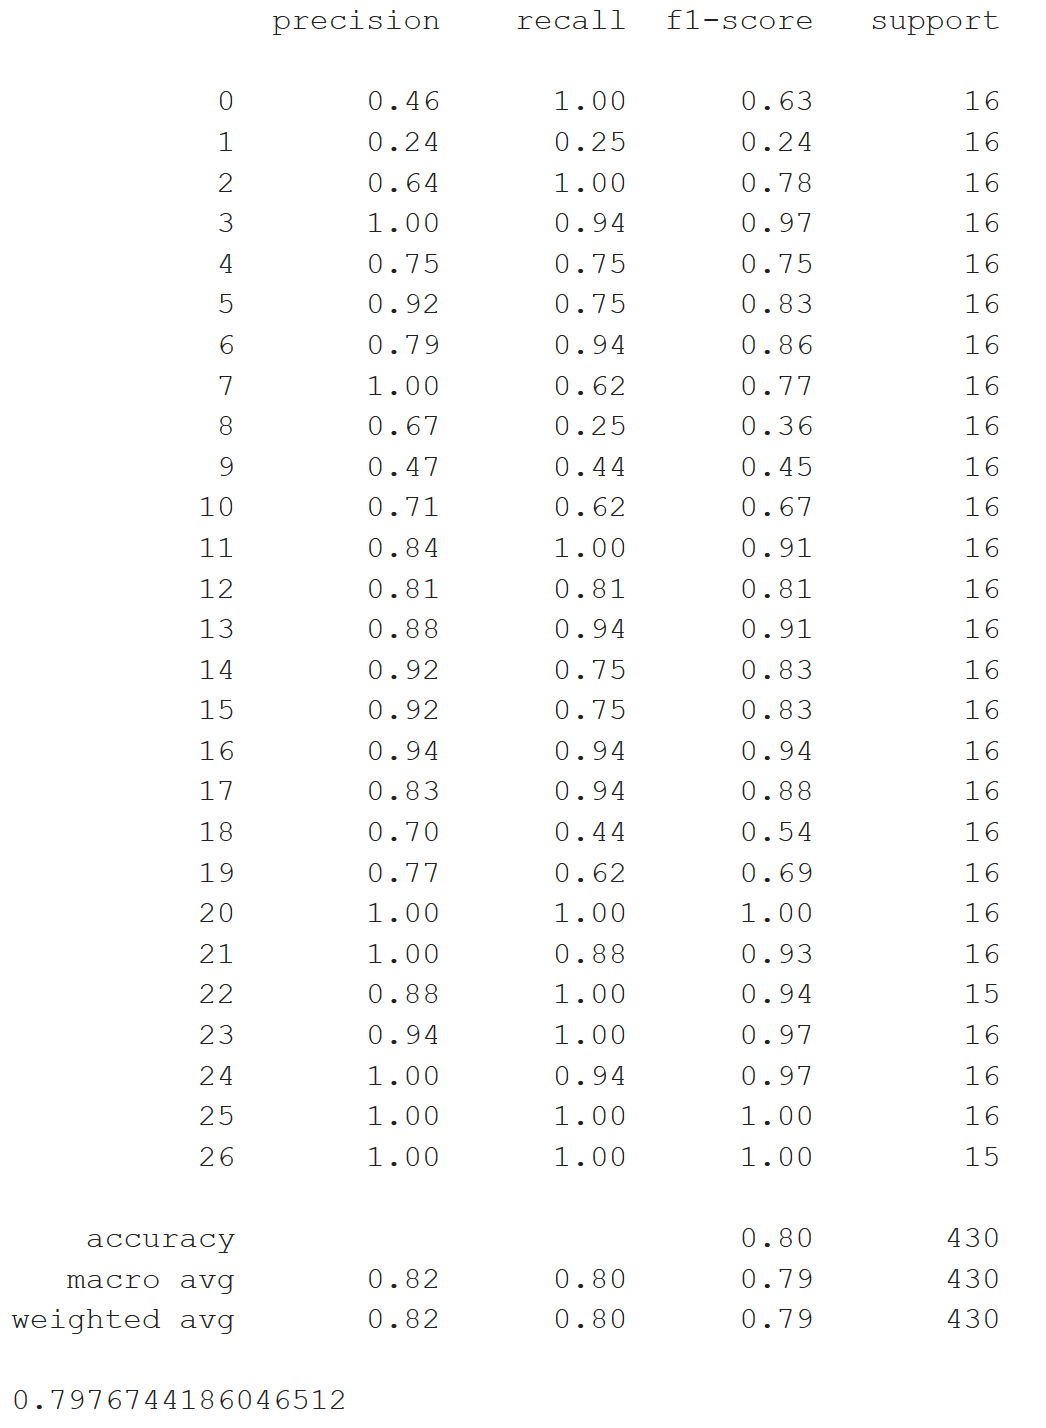
\includegraphics[scale=0.55]{Image/rf_27_class_report.png}
\caption{\label{rf_27_class_report} Classification Results for Random Forest}
\end{center}
\end{figure}

\begin{figure}[H]
\begin{center}
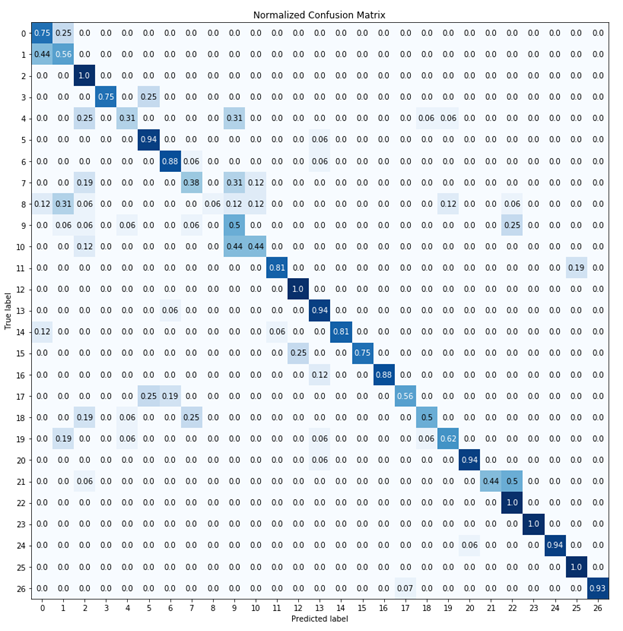
\includegraphics[scale=1]{Image/rf_27_class_confusion.png}
\caption{\label{rf_27_class_confusion} Confusion Matrix for Random Forest}
\end{center}
\end{figure}

\subsection{Gradient Boosted Trees with Xgboost}

When Xgboost was applied to the same dataset, an accuracy of 67.67 percent was achieved. It was observed that class 7 and 8 have the worst f1-score of 0.27. From the confusion matrix, it was observed that class 1 again was easily confused with class 0 (0.32 vs 0.62). Similarly for class 7 and 8, there were large portions of mis-classifications but spread to more classes. For example, for class 7, it was most confused with class 9 as well as class 10 and 18 to a lesser extent.

\begin{figure}[H]
\begin{center}
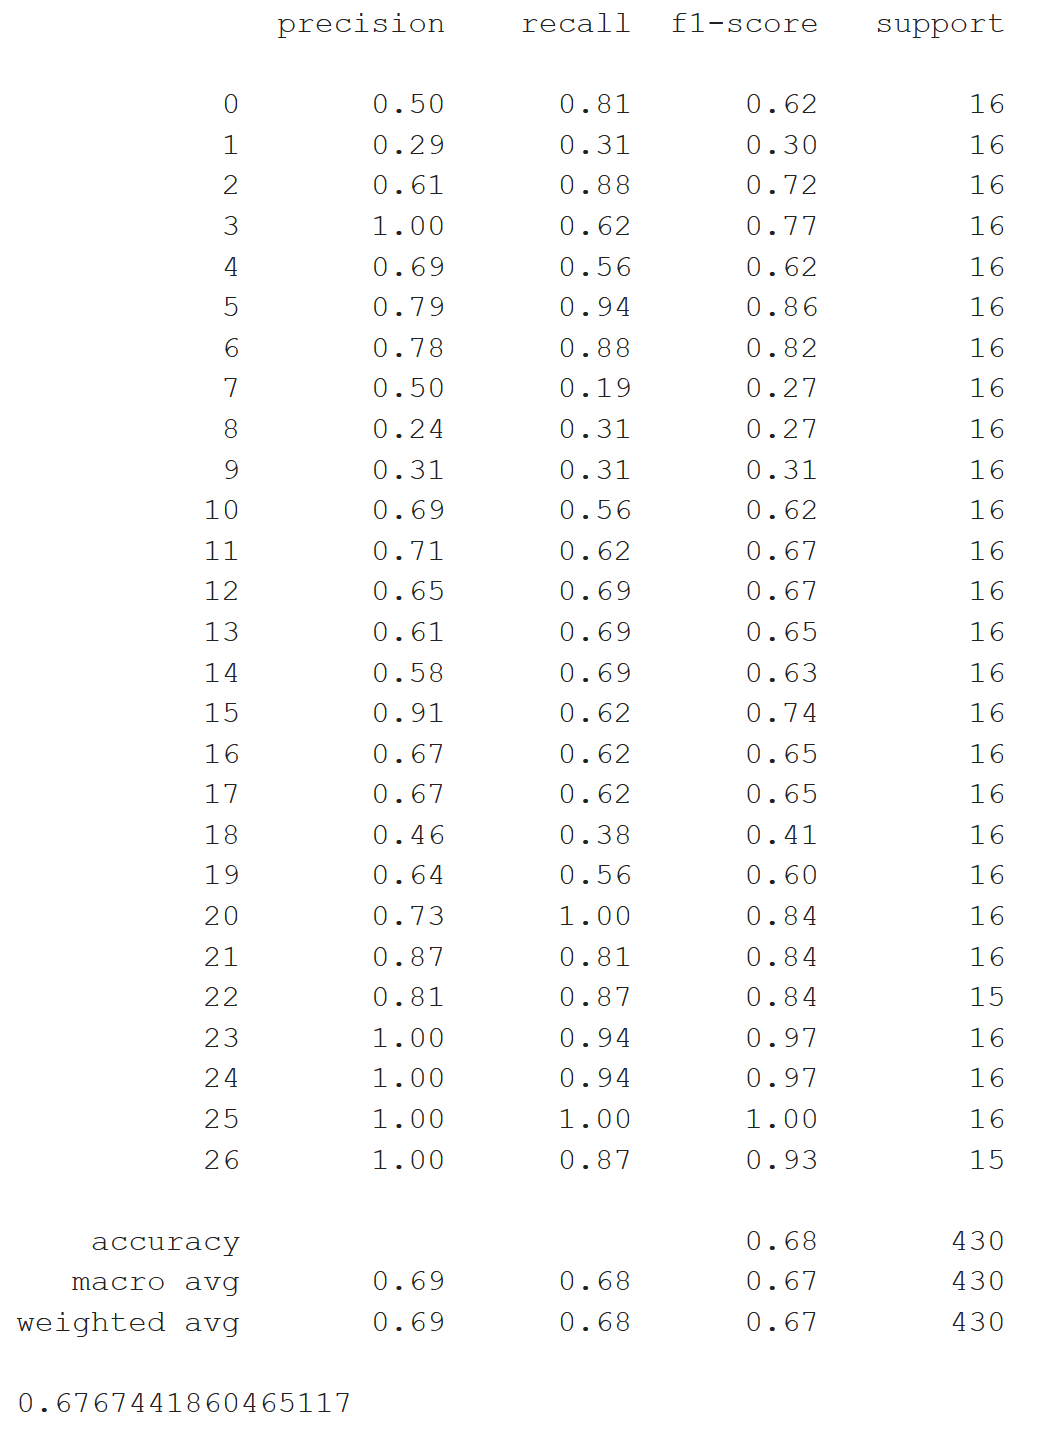
\includegraphics[scale=0.55]{Image/xgb_27_class_report.png}
\caption{\label{xgb_27_class_report} Classification Results for Xgboost}
\end{center}
\end{figure}

\begin{figure}[H]
\begin{center}
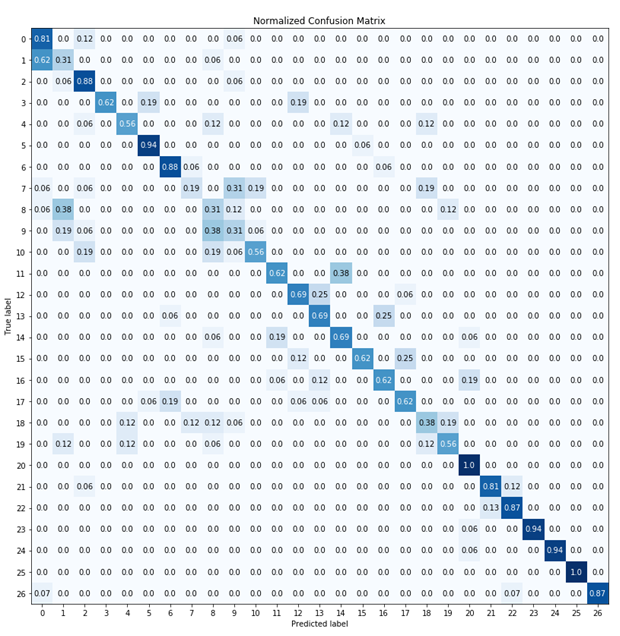
\includegraphics[scale=1]{Image/xgb_27_class_confusion.png}
\caption{\label{xgb_27_class_confusion} Confusion Matrix for Xgboost}
\end{center}
\end{figure}

\subsection{Convolutional-1D Neural Network}

Despite the Convolutional-1D Neural Network achieving a higher accuracy of 69.30 percent when compared to Xgboost, it was observed that class 8 has a f1-score of 0. From the confusion matrix, this class is commonly mis-classified as class 0, 1, 9 or 10. However this model has the highest f1-score for class 1 amongst the 3 models.

\begin{figure}[H]
\begin{center}
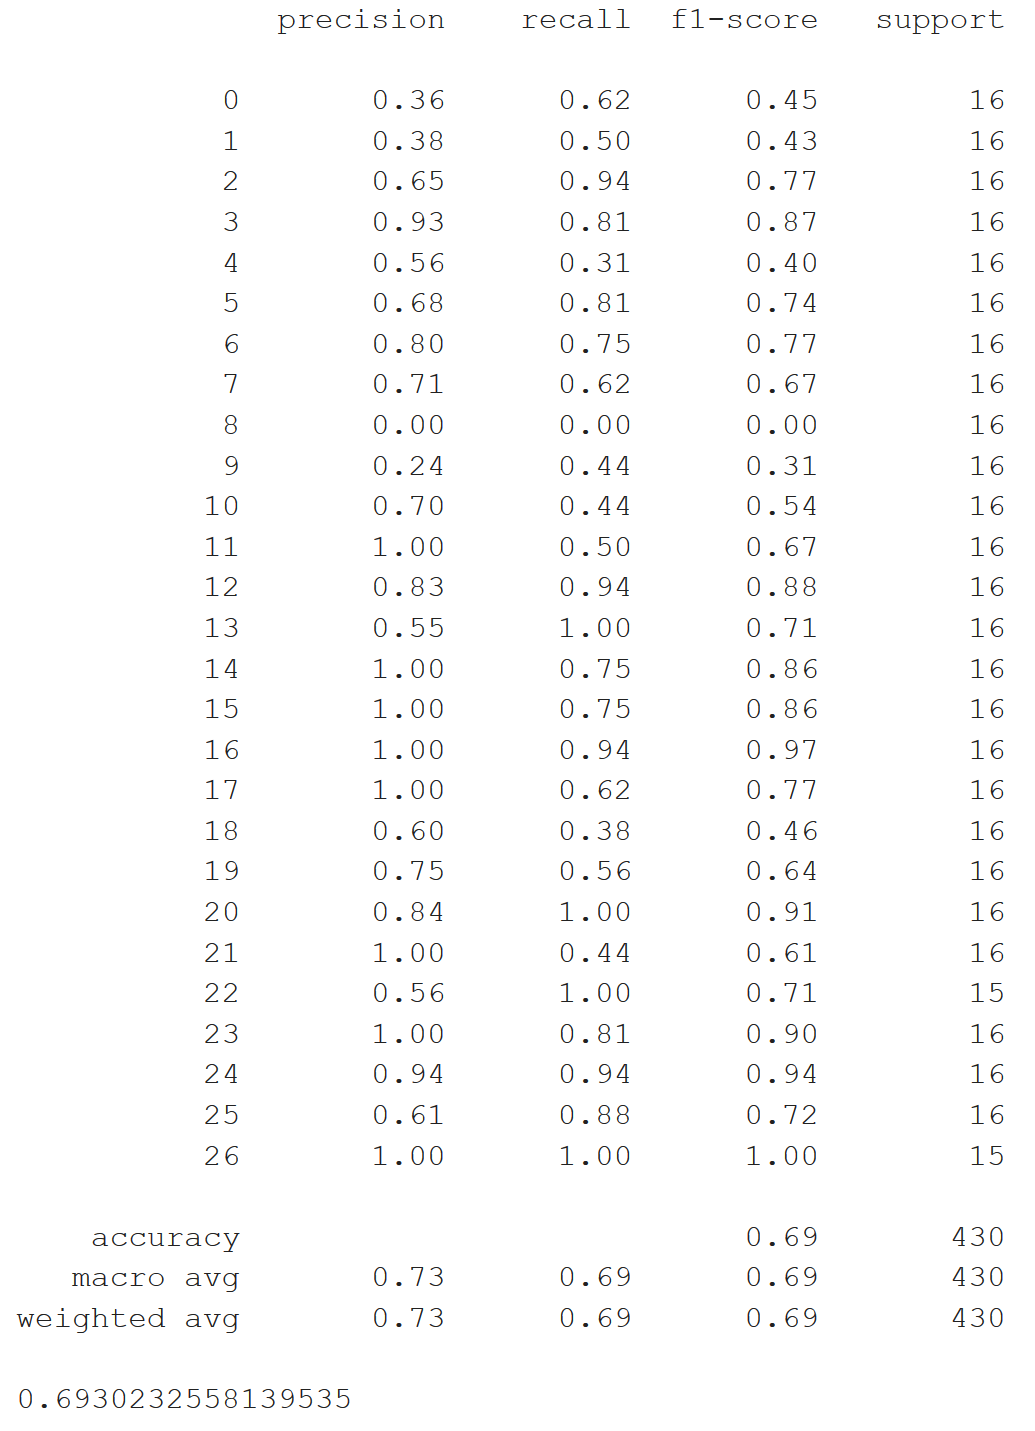
\includegraphics[scale=0.55]{Image/cnn1d_27_class_report.png}
\caption{\label{cnn1d_27_class_report} Classification Results for Convolutional-1D Neural Network}
\end{center}
\end{figure}

\begin{figure}[H]
\begin{center}
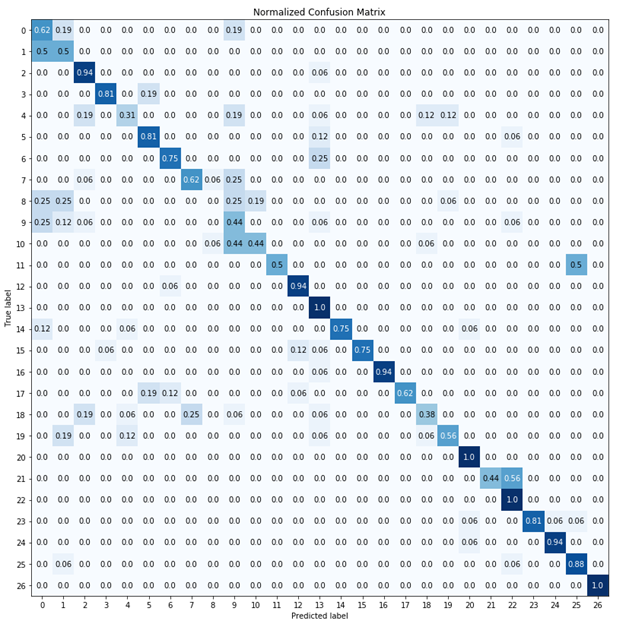
\includegraphics[scale=1]{Image/cnn1d_27_class_confusion.png}
\caption{\label{cnn1d_27_class_confusion} Confusion Matrix for Convolutional-1D Neural Network}
\end{center}
\end{figure}

\subsection{Voting Multi-classifier}

Observing that the previous 3 models had varying levels of performance for different classes. A voting multi-classifier of Random Forest, Xgboost and Convolutional-1D Neural Network was built. However the accuracy of this voting classifier was lower than that of Random Forest at 72.56 percent. This model also suffers greatly for class 8 at a f1-score of 0. Class 1 is still most confused with class 0 (0.56 vs 0.44).

\begin{figure}[H]
\begin{center}
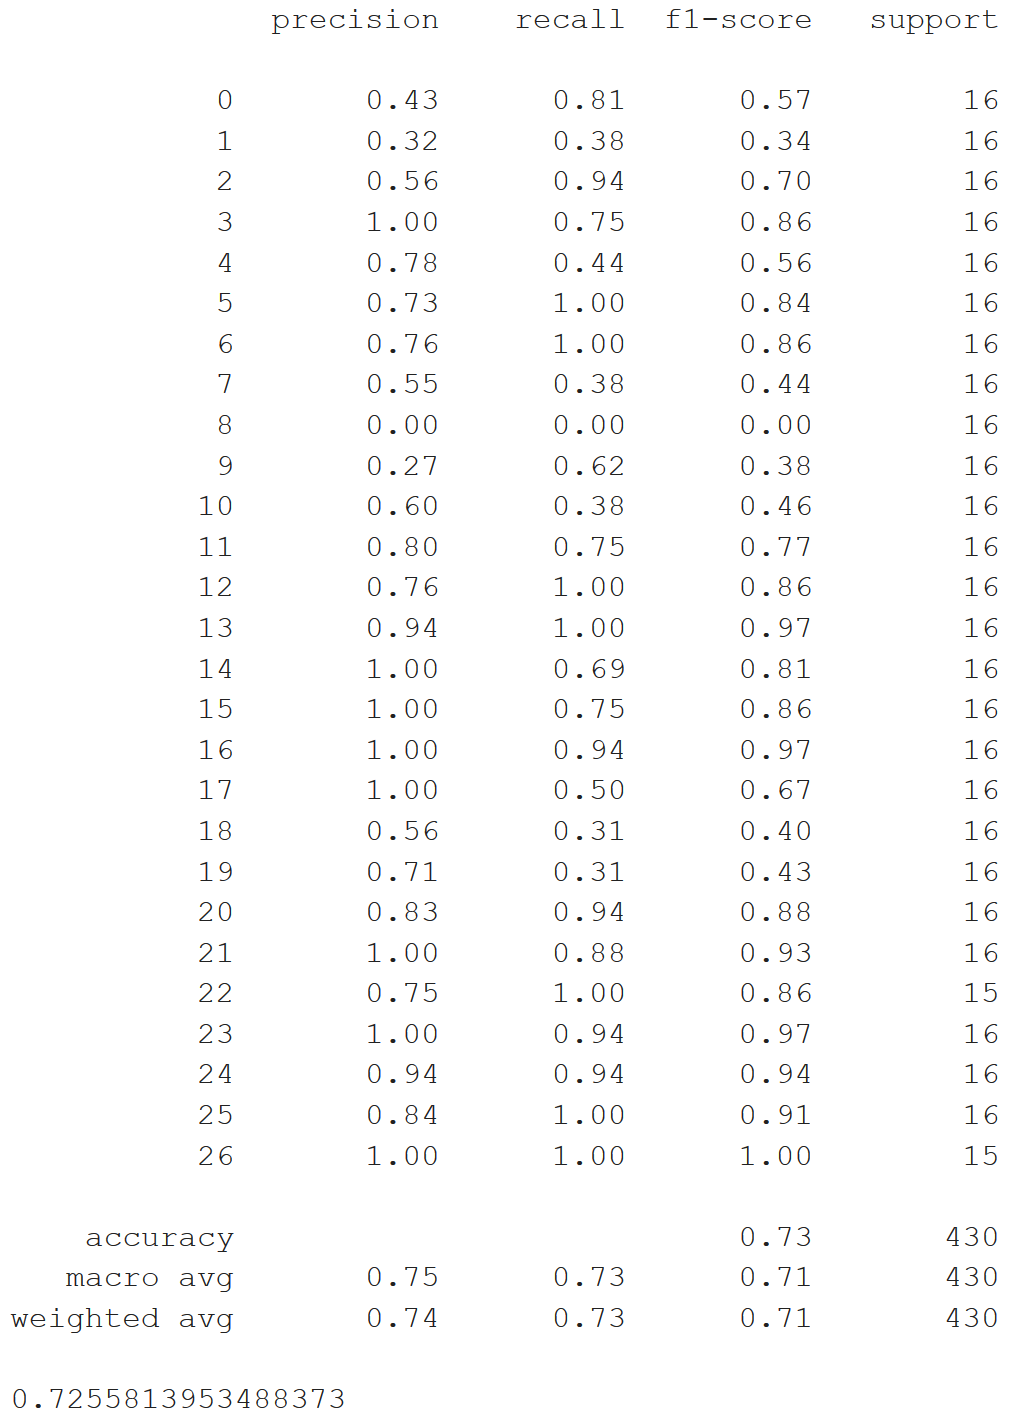
\includegraphics[scale=0.55]{Image/vote_27_class_report.png}
\caption{\label{vote_27_class_report} Classification Results for Voting Multi-classifier}
\end{center}
\end{figure}

\begin{figure}[H]
\begin{center}
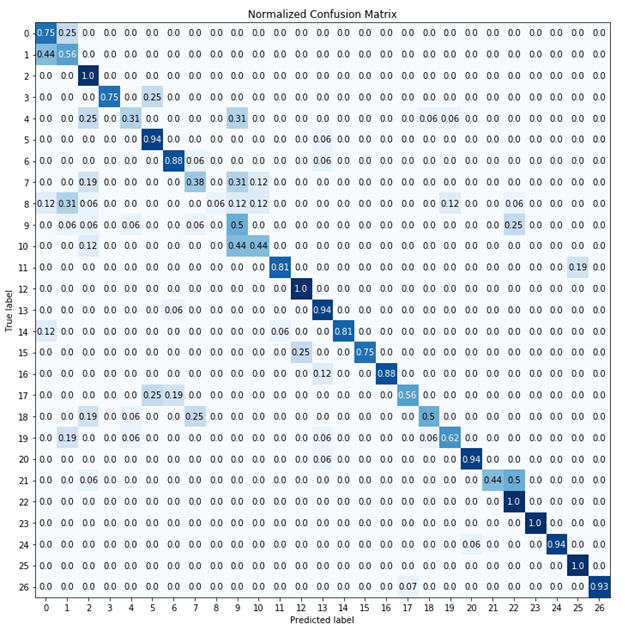
\includegraphics[scale=1]{Image/vote_27_class_confusion.png}
\caption{\label{vote_27_class_confusion} Confusion Matrix for Voting Multi-classifier}
\end{center}
\end{figure}

\subsection{Comparison of Machine Learning Models}

Table \ref{tbl:compare_ml} shows a comparison of the accuracy of the various models.
\begin{table}[H] 
\begin{center}
\caption{Performance Comparison for different Machine Learning Models} \label{tbl:compare_ml}
\begin{tabular}{|c|c|c|c|}
\hline
Imaging Method & Accuracy \\
\hline
Random Forest  & 79.77  \\
\hline
Xgboost & 67.67  \\
\hline
Convolutional-1D Neural Network & 69.30  \\
\hline
Voting Multi-Classifier & 72.56  \\
\hline
\end{tabular}
\end{center}
\end{table}

From this, it can be seen that the Random Forest Classifier is the best amongst the models built so far.

\section{Long Short Term Memory Model}

A LSTM model with Conv 1D was built to learn the temporal pattern in the dataset. The model consist of 4 Conv1D layers, 2 LSTM layers and 1 Dense layer with Softmax activation function as shown in fig \ref{fig:LSTM_Model}. The purpose of the Conv1D layers is to perform feature extraction. ReLU activation function was used for all the Conv1D layers. Dropout was added at the LSTM layers to avoid overfitting. Learning rate was set to 1e-4 with a decay of 1e-6 using Adam Optimizer and batch size was set to 4. 

\begin{figure}[H]
\begin{center}
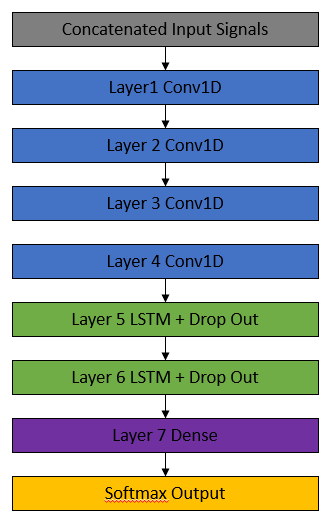
\includegraphics[scale=0.8]{Image/LSTM_Model.png}
\caption{\label{fig:LSTM_Model} Conv1D + LSTM Model}
\end{center}
\end{figure}
 
 Inertial sensor signal and the feature engineered Skeleton Joint Angle signal was re-sampled to a common length and fed into the Conv1D + LSTM Model. The Model achieved an accuracy of 80.69 percent.
 
 \begin{figure}[H]
\begin{center}
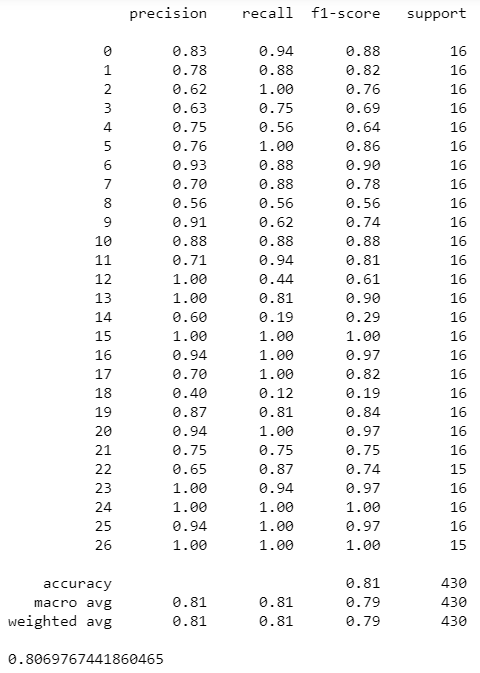
\includegraphics[scale=0.8]{Image/LSTM_Accuracy_Scores.png}
\caption{\label{fig:LSTM_Accuracy_Scores} Accuracy Scores}
\end{center}
\end{figure}

\begin{figure}[H]
\begin{center}
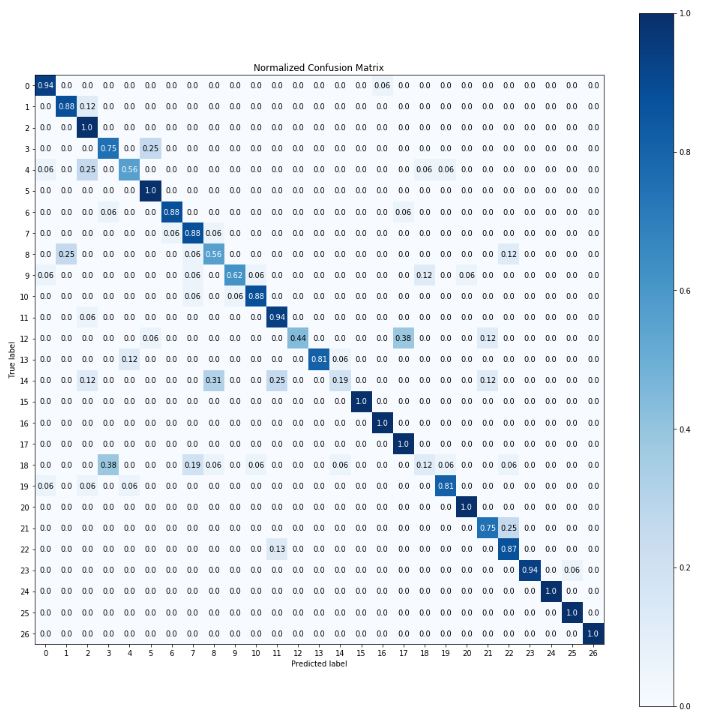
\includegraphics[scale=0.6]{Image/LSTM_Confusion_Matrix.png}
\caption{\label{fig:LSTM_Confusion_Matrix} Confusion Matrix}
\end{center}
\end{figure}
 
\section{New Graph Machine Learning Model}

A new graph machine learning model was conceptualised and implemented to exploit the feature engineered Joint Sequence data. 
\subsection{Model Architecture}

The nodes in the graph is made up of joints which represents activation of a specific joint. The number of nodes for each joint depends on the number of times it is activated through the same sequence. The directional link between the nodes represent an activation sequence (e.g. A,B means Joint B was activated after Joint A was activated) and the weight of the link represents the frequency of activation. A separate graph is generated for each of the classification classes. For this dataset, 27 graphs were generated. 

\subsection{Training the Model}

To train the model, each sequence in the training data is used to update the weight of the link in the graph of its specific class. The training process is illustrated using three training data. \\

Training Data 1: A,B,C,D,A

\begin{figure}[H]
\begin{center}
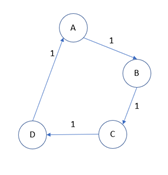
\includegraphics[scale=1]{Image/Graph1.png}
\caption{\label{fig:Graph1} Graph After One Training Sequence}
\end{center}
\end{figure}

When a repeated sequence pair appears in a single sequence, a new node will be created and the weight to the new node will be updated. This is to account for the multiple occurrence of same pairwise joint activation. In the example below, A,B occurred during the first, fifth and ninth sequence and therefore B2 and B3 node was created. B,A occurred during the eighth and tenth sequence and therefore A2 node was created.\\

Training Data 2: A,B,C,D,A,B,E,B,A,B,A

\begin{figure}[H]
\begin{center}
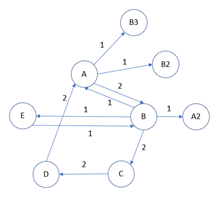
\includegraphics[scale=1]{Image/Graph2.png}
\caption{\label{fig:Graph2} Graph After Two Training Sequence}
\end{center}
\end{figure}

It is also possible for the same joint to be activated after itself. Think of just moving the elbow up and down without moving other joints. \\

Training Data 3: B,C,D,A,B,A,A,A

\begin{figure}[H]
\begin{center}
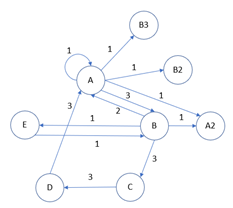
\includegraphics[scale=1]{Image/Graph3.png}
\caption{\label{fig:Graph3} Graph After Three Training Sequence}
\end{center}
\end{figure}

One point to note is that when updating the weights, the sequence always originates from the primary nodes (nodes without suffix). 

\subsection{Classifying }

To determine which class a sequence belongs to, the sequence is scored using all the graphs and is classified as the class it has obtained the highest score from. Using the same graph in Fig. \ref{fig:Graph3} as example (assuming it has been trained), three unseen sequence was scored and the calculation as shown in table \ref{tbl:basic_score} below. Noticed that the first 2 sequences are extracted and slightly modified from the training data and the 3rd sequence is randomly created. This is the basic scoring without bonus combo score and is not the final score yet. 

\begin{table}[H] 
\begin{center}
\caption{Basic Scoring} \label{tbl:basic_score}
\begin{tabular}{|c|c|}
\hline
Sequence & Score \\
\hline
A,B,C,D,A,E,B  & 3+3+3+3+0+1=13  \\
\hline
C,D,A,B,A,A,B & 3+3+3+2+1+1=13  \\
\hline
C,B,A,D,A,E,A & 0+2+0+3+0+0=5  \\
\hline
\end{tabular}
\end{center}
\end{table}

To score for similarity beyond pairwise sequence, a bonus combo score is added to the base score according to the formula below. 

\begin{equation}
Bonus = (no. of consecutive match – 1) X b
\end{equation}
Where b is the bonus multiplier. \\

Continuing from the same example, the bonus score was calculated in table \ref{tbl:total_score} below. It can be seen that applying the bonus score (setting b=2) further differentiates the sequence that does not belong to the class. 

\begin{table}[H] 
\begin{center}
\caption{Bonus Scoring} \label{tbl:total_score}
\begin{tabular}{|c|c|c|c|}
\hline
Sequence & Score & Bonus Score & Total Score\\
\hline
A,B,C,D,A,E,B  & 13 & 4 & 17  \\
\hline
C,D,A,B,A,A,B & 13 & 8 & 21  \\
\hline
C,B,A,D,A,E,A & 5 & 0 & 5  \\
\hline
\end{tabular}
\end{center}
\end{table}

Lastly, the total score will be weighted according to its sequence length against the average sequence length in the class to produce the final score. This is to distinguish between classes with similar sequence pairs but different sequence length (e.g. waving vs swap left).

As a demonstration, the model was trained and tested with 5 selected actions and has achieved a reasonably high accuracy of 92.41 percent.\\ \\
The 5 selected actions are:

\begin{enumerate}
\item Right arm swipe to the left
\item Basketball Shoot
\item Right hand pick up and throw
\item Jogging in place
\item Squat
\end{enumerate}

\begin{figure}[H]
\begin{center}
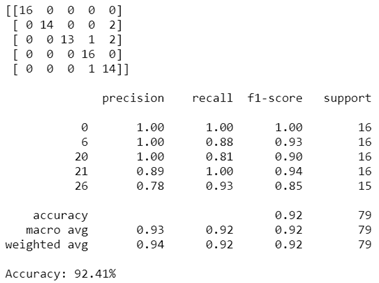
\includegraphics[scale=1]{Image/Graph_Model_Accuracy.png}
\caption{\label{fig:Graph_Model_accuracy} Classification Results for 5 Actions}
\end{center}
\end{figure}

However, when apply to classify all 27 actions, it was only able to achieve about 30 percent accuracy which is still much better than random guess of 3.7 percent (100 percent/27). The model is still in early stage of development and stated below under future explorations are some enhancements to improve the model. 

\subsection{Future Explorations}

\subsubsection{Reciprocal Weight Update}

It was observed that some joint activation occurred in close proximity with each other and sometimes one occurs before another. Borrowing the idea from self-organising map (SOM), when the weight for a link between 2 nodes are updated, the weight of the reciprocal link is also updated with a fraction of the weight update value. For example, when A,B link is updated by a value of 1, B,A is updated by a value of 0.5.

\subsubsection{Amplitude Matching}

In the current design of the model, amplitude value is not considered when scoring a sequence according to a graph. During model training, the average amplitude value could be computed and stored at each link. When scoring, the score given between 2 nodes would be a percentage of the weight value corresponding to the percentage match between the average amplitude and the amplitude of the sequence being scored. 

\subsubsection{Iterative Training}

The current training process of the model is one pass. One possible iterative training approach is to increase the weight update magnitude of wrongly classified sequences to increase the representation of their signature in the graph of their class.

\subsection{Suitability for Other Use Cases}

This new graph model is suitable for solving problems with sequential peak data such as equipment fault prediction based on multiple sensor data and animal recognition, behaviour prediction and health monitoring by training the model to recognise the animal’s movement.  

\section{Encoding Time Series to Images for Classification}

\subsection{Overview of Approach}
In 2015, Wang et al has demonstrated the effectiveness of converting time series signals into images for use of classification using Tiled Convolutional Neural Networks through the use of Gramian Angular Field \cite{inproceedings}. Later on in 2016, Liu et al demonstrated the effectiveness of visualizing and mining data with the use of Markov Transition Field \cite{liu2016encoding}.

Hatami et al then further demonstrated in their 2017 paper that the use of Recurrence Plots and Deep Convolutional Neural Networks offer a competitive approach to handle time-series and sequences \cite{hatami2017classification}.

The common theme across the 3 papers is the conversion of 1D signals into 2D matrices through various methods like the conversion to polar coordinate system (Gramian Angular Field), quantization and the generation of Markov Matrix (Markov Transition Field) and the generation of R-Matrix (Recurrence Plots). After the generation of these images, they are fed into a Convolutional-2D Neural Network commonly used in Computer Vision.

These images can be generated using the pyts package by Faouzi et al \cite{johann_faouzi_2019_2561773}. Examples of such generated images are illustrated in the figure below, which are taken from the documentation of the pyts \cite{johann_faouzi_2019_2561773} package.

\begin{figure}[H]
\begin{center}
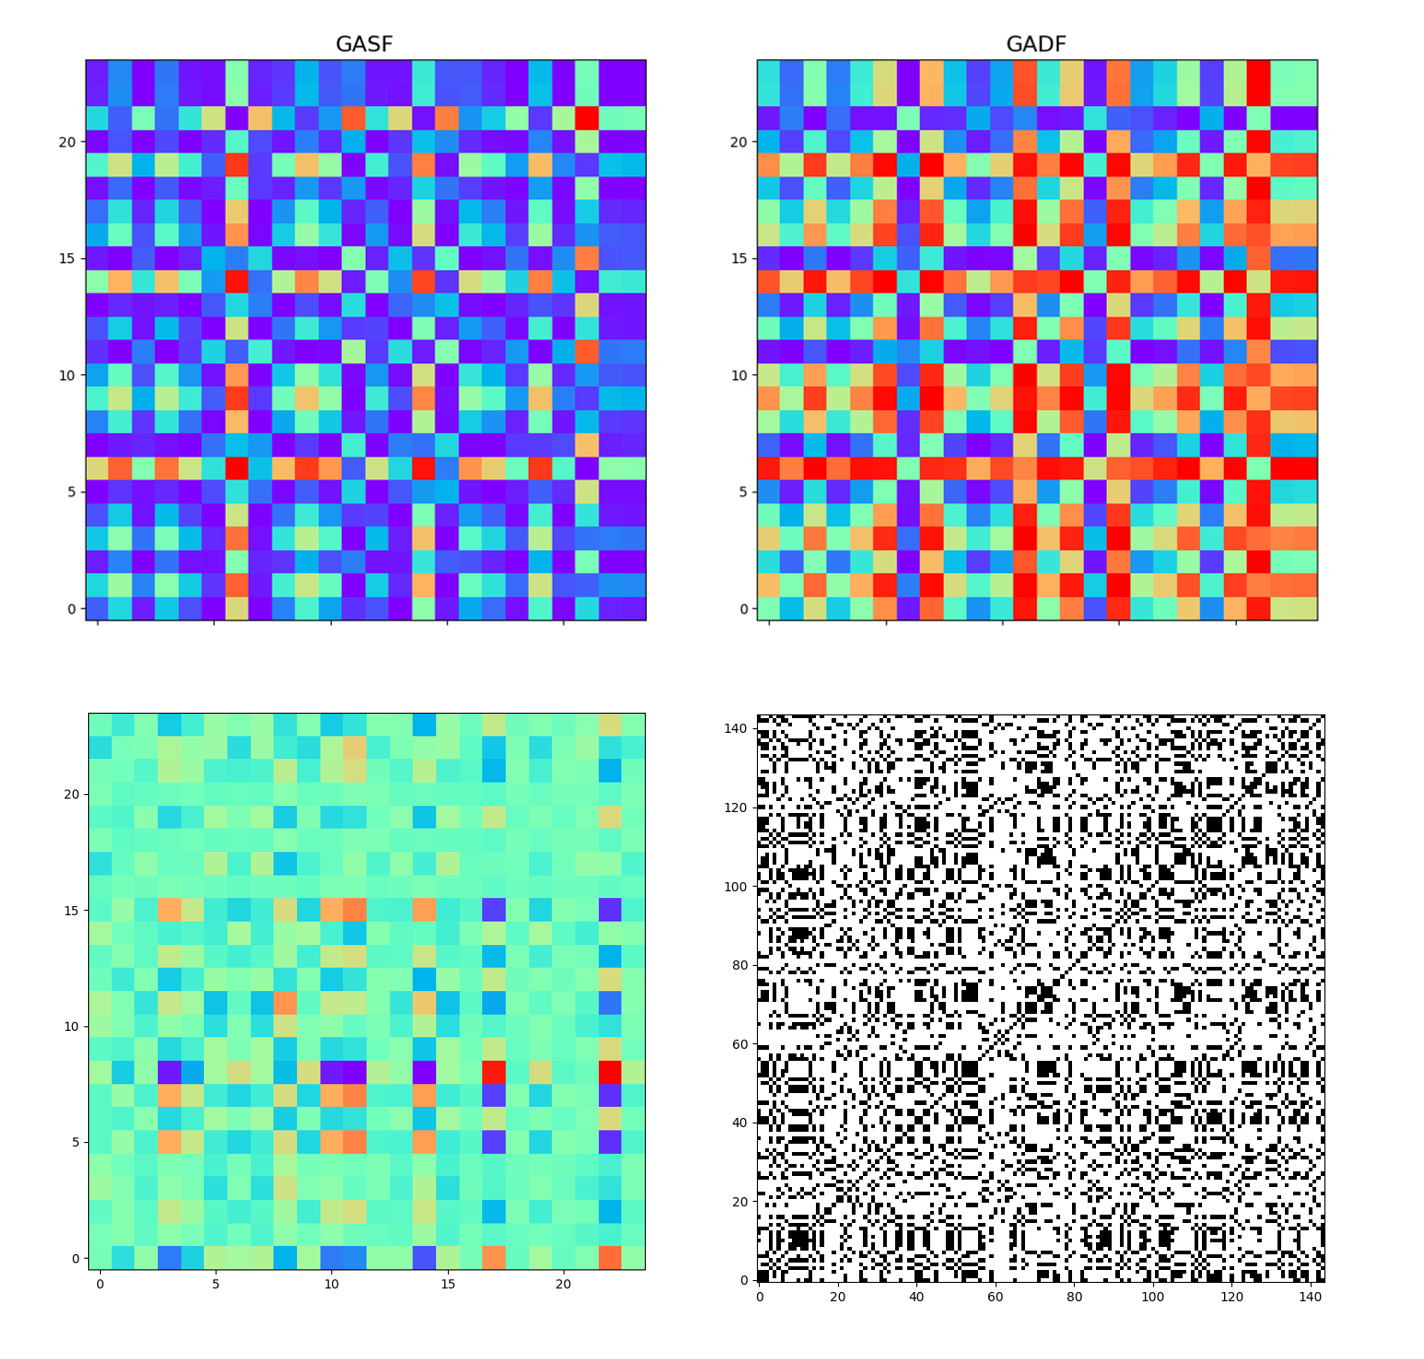
\includegraphics[scale=0.5]{Image/ts_to_img_sample.png}
\caption{\label{ts_to_img_sample} Sample output from pyts package documentation. Top Left: Gramian Angular Summation Field, Top Right: Gramian Angular Difference Field; Bottom Left: Markov Transition Field, Bottom Right: Recurrence Plots}
\end{center}
\end{figure}

\subsection{Application to Dataset}
Before transformation a sample of the the combined variance and angle sequences extracted from inertial and skeleton sequences is shown below.

\begin{figure}[H]
\begin{center}
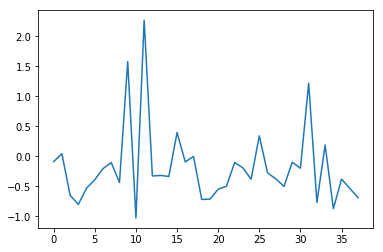
\includegraphics[scale=0.5]{Image/ts_before_img.png}
\caption{\label{ts_before_img} A single sample from Training Data}
\end{center}
\end{figure}

Individual image generation methods and additional selected combinations were also attempted such as overlaying and merging different plots into a single image as well as placing plots generated side-by-side into a square grid. In total the six types of image methods below and their corresponding pixel size are selected.

\begin{enumerate}
\item Gramian Angular Difference Field (38x38)
\item Gramian Angular Summation Field (38x38)
\item Markov Transition Field (38x38)
\item Recurrence Plot (38x38)
\item Overlay of Gramian Angular Difference Field and Recurrence Plot (38x38)
\item Combination of item 1 to 4 in a 2x2 grid (76x76)
\end{enumerate}

An example of the generated images from training data using the Recurrence Plot method is shown below. Each small grid in the image represents a generated image from the stated class label. In particular, looking at the 2 pairs of images from classes 8 and 24, it can be observed that the samples have distinct image patterns, providing intuition that some learning can be achieved from these generated images.

These images are then saved according to their techniques applied and corresponding and class labels. Converter functions are fitted to training data and the same fitted functions are applied to both training and testing dataset.


\begin{figure}[H]
\begin{center}
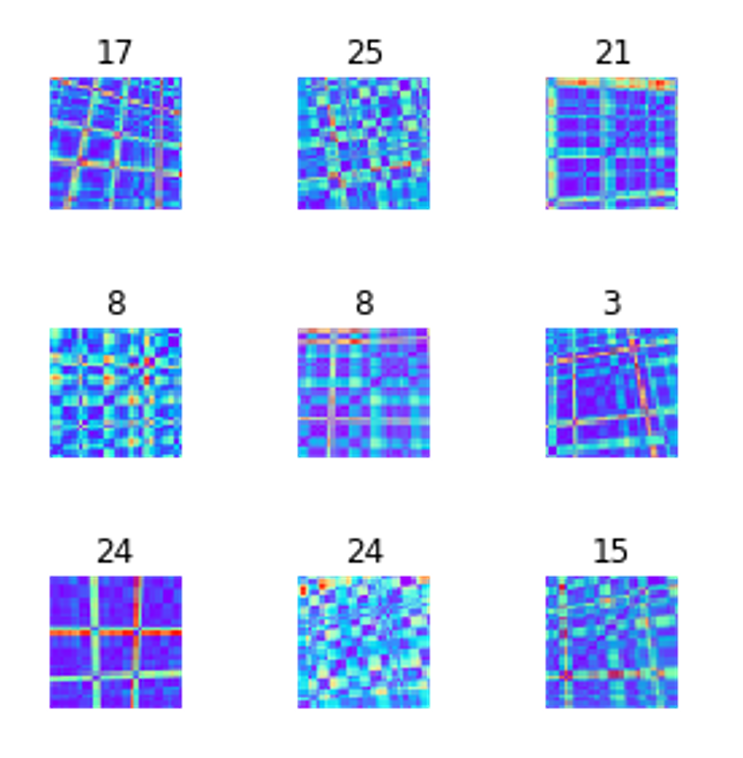
\includegraphics[scale=1]{Image/recurrence_plot_augmented.png}
\caption{\label{recurrence_plot_augmented} A sample batch of Recurrence Plots generated from Training Data}
\end{center}
\end{figure}

A particular point to note regarding the above figure is that it shows the the images with Train-Time Image Augmentation already applied to them. Only Image Transforms like zoom, shears and rotation are applied. No horizontal and vertical flips are performed as these are not as applicable for this dataset.

\subsection{Model Selection and Transfer Learning}
Dense Convolutional Network (DenseNet) are chosen as they are found to perform well on small datasets by Huang et al \cite{huang2016densely}. A key architecture highlight from the paper is that DenseNet connects each layer to every other layer in a feed-forward fashion, where each network has L(L+1)/2 direct connections. Within each layer, the feature-maps of all preceding layers are used as inputs, and its own feature-maps are used as inputs into all subsequent layers. A summary of the DenseNet architecture reproduced from the paper is shown in the diagram below. In particular, for this assignment, the DenseNet-121 version has been chosen.

\begin{figure}[H]
\begin{center}
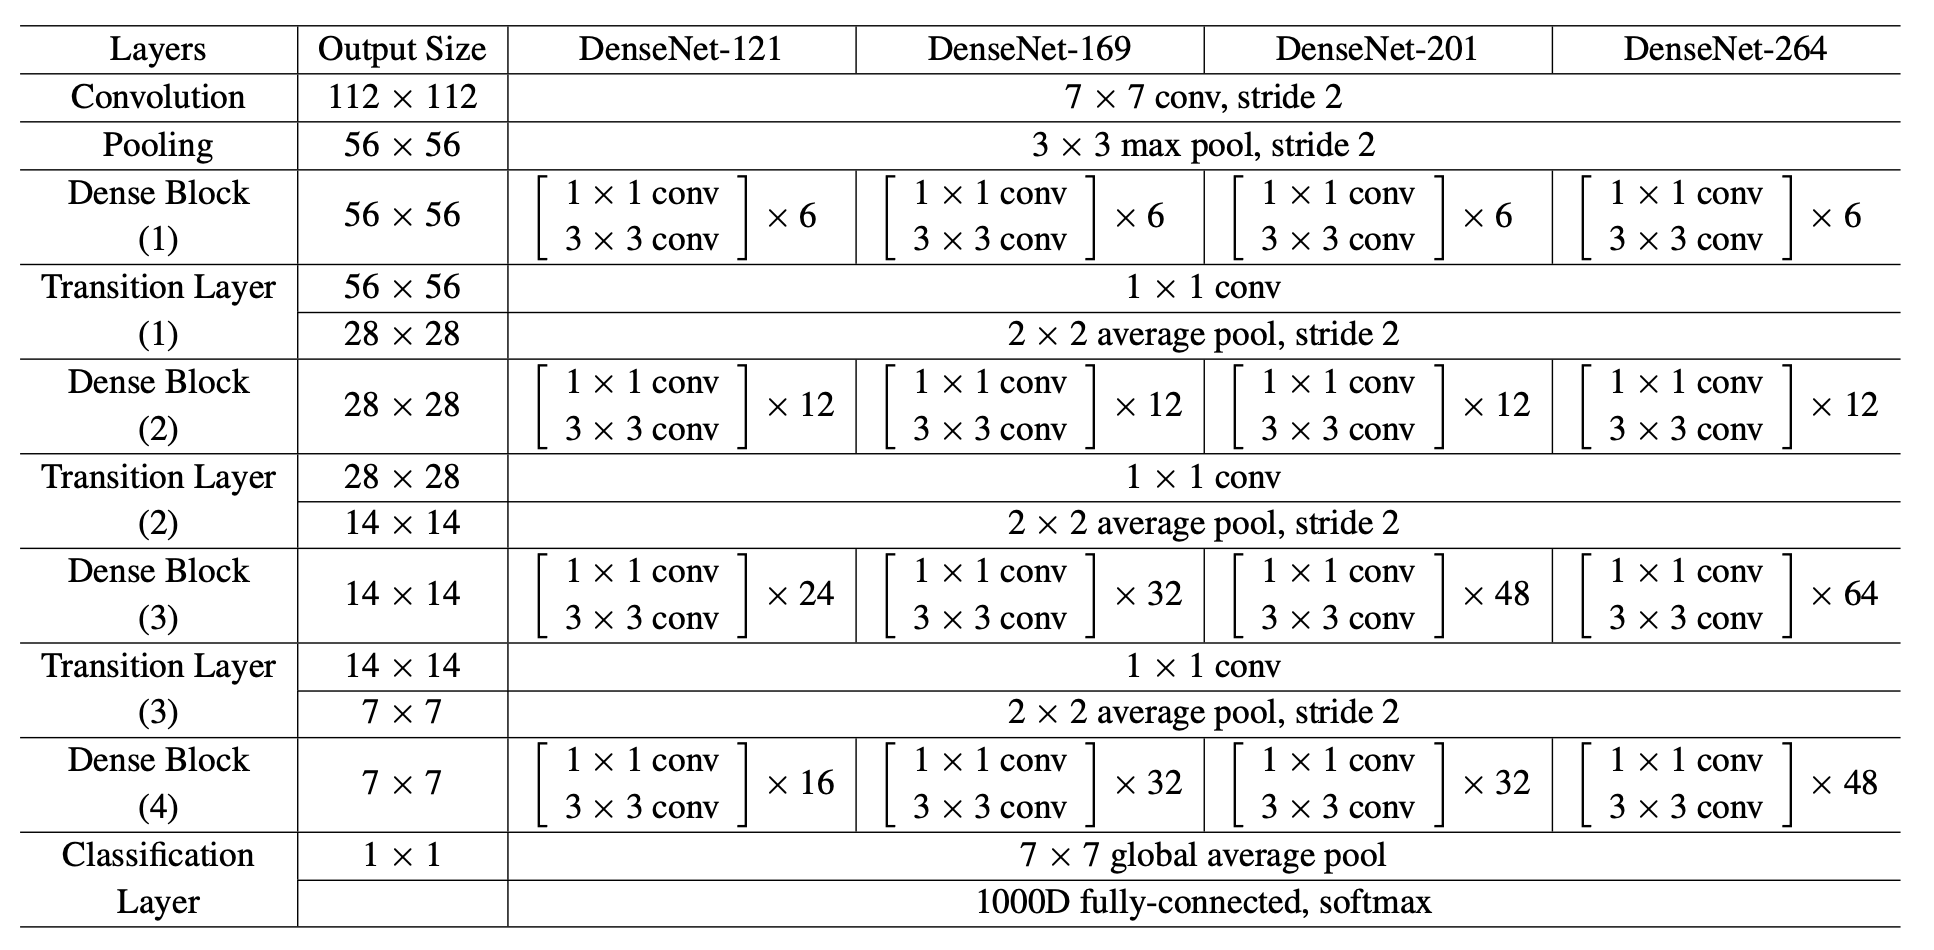
\includegraphics[scale=0.27]{Image/densenet2.png}
\caption{\label{densenet} DenseNet Architecture from the paper by Huang et al}
\end{center}
\end{figure}

Selection of this architecture fits the profile of the dataset very well since there are only 861 observations for 27 classes. In addition, the image generated are only 38-by-38 pixels in size.

To enable quick iteration and proving of the effectiveness of the method, the team decided to leverage on adapting and fine-tuning pre-trained DenseNet-121 models. Transfer Learning is performed using the PyTorch-based fastai package by Howard et al \cite{howard2018fastai}

Transfer learning is performed in two stages. In the first stage, the base DenseNet model is not trained or freezed. Only the added fully connected 512 hidden units layer and final 27-class output layer is trained for 50 epochs.

Subsequently, the base model is unfreezed and the whole model is trained for another 50 epochs. This is also known as the finetuning phase.

\subsection{Results of Approach}
After running transfer learning for the six types of image generation (individual/combined) methods, table \ref{tbl:compare_cnn} below provides an overview of the results.

\begin{table}[H] 
\begin{center}
\caption{Performance Comparison for different imaging methods} \label{tbl:compare_cnn}
\begin{tabular}{|c|c|c|c|}
\hline
Imaging Method & Accuracy \\
\hline
Gramian Angular Difference Field (GADF)  & 40.70  \\
\hline
Gramian Angular Summation Field (GASF) & 37.44  \\
\hline
Markov Transition Field (MTF) & 11.40  \\
\hline
Recurrence Plot (RP) & 45.58  \\
\hline
GADF + RP Overlay & 21.63  \\
\hline
GADF + FASF + MTF + RP side-by-side quadrant & 43.95  \\
\hline
\end{tabular}
\end{center}
\end{table}

It has been observed that the Recurrence Plot method achieved the highest accuracy amongst the methods attempted. The highest accuracy achieved is 45.58 percent. This is lower than other approaches but still much better than random guess.

Upon a closer look at the confusion matrix below, it has been observed that some classes like classes 1 and 2 are severely mis-classified. In particular for class 1, the largest portion is being mis-classified as class 0. Further explorations can be made in future on to how this approach can be refined given more time.

\begin{figure}[H]
\begin{center}
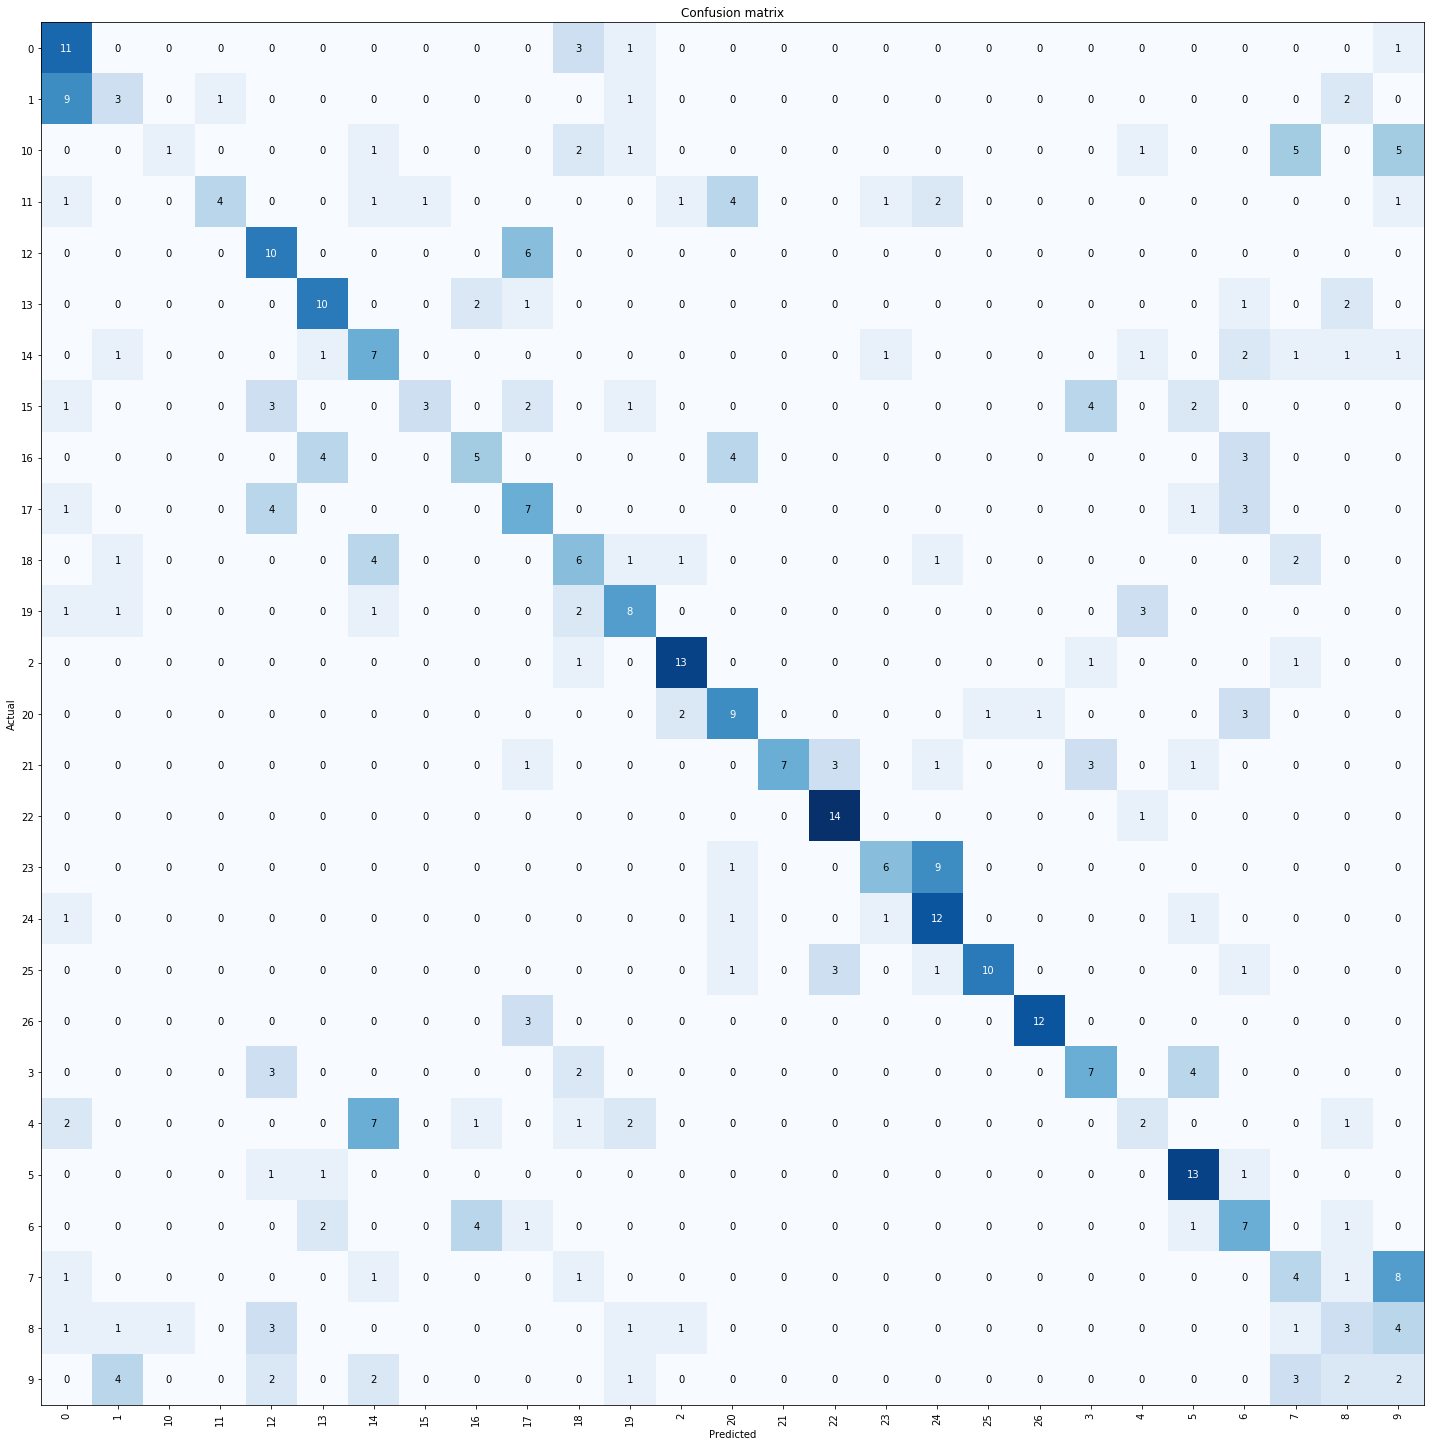
\includegraphics[scale=0.15]{Image/rp_confusion.png}
\caption{\label{rp_confusion} Confusion Matrix of Best Model using Recurrence Plots}
\end{center}
\end{figure}


\section{Findings and Conclusion}

Through understanding the classification task and the features in the dataset, the team has performed relevant feature engineering and successfully built two different models that outperformed the benchmark accuracy of 79.1 percent. The Random Forest model has an accuracy of 79.77 percent and the Conv1D + LSTM model has an accuracy of 80.69 percent.

The team went further to conceptualise and implement a new graph machine learning model which has achieved an accuracy of 92.41 percent classifying 5 selected actions. 

Lastly, the team also explored encoding the time series data into images and leveraged on transfer learning to train the classifier. At the moment, this technique is not mature for general application and has only achieved an accuracy of 45.58 percent.

To further improve the accuracy in the task of classifying human actions, future exploration works could include more advanced feature engineering and incorporating rule based system to assist in differentiating between very similar actions that machine learning models could not tell apart.

\bibliographystyle{IEEEtran}
\bibliography{bibfile}
\end{document}